\section{Software: Governing machine protocols and stimulus presentation}
\label{sec:sectionc}

Bpod's software allows to load user-made protocols and run them within the built-in bpod interface, joined with the protocols' specific GUI windows (IMAGE).

In this project, three protocols were developed for different ends: receptive field mapping, tuning measuring and studying the spatial structure of surround modulation.

Each of these were subsequently used in mice experiments. The produced data was also analysed, validating the method and tool in the three protocols. 

The RF protocol served to find the RF positions after each experimental session and assess if the majority of the measured cells' RFs was centred at the corresponding display monitor center, as desired. Specifically, the obtained RF maps either indicated, in combination with the retinotopy maps, in which directions one should move the objective to correct the imaging position in following sessions or confirmed that the objective and mouse placing was appropriate (SEE CHAPTER). Furthermore, this data was also combined with the SM protocol's results for RF position-dependent analysis of the SM effect (SEE CHAPTER).

The tuning protocol was implemented to measure the selectivity of cells in a flexible array of conditions. The data collected from this protocol was analysed and some cell's tuning behaviour examples are shown in (SEE CHAPTER). This analysis served to validate the protocol and aided in troubleshooting the SM analysis. Moreover, this protocol was also used to find the RF centred imaging positions during experiments. 

Finally, the SM study was the main focus of this project's experimental component, and the obtained results are presented in (SEE CHAPTER). The implementation of this protocol allows the presentation of any configuration with center and surround moving gratings' patches, in any combination of the four cardinal plus center positions. For this project's purposes, 124 were chosen, in a given set of grating frequencies and stimuli sizes (SEE CHAPTER).

Each of these protocols follows a similar structure of five files, each with different case functions:

\begin{itemize}
\item \textbf{main}: initiate, submit, start, prepare next trial, synchronize GUI, save settings and events, process trial completed, restart and stop;
\item \textbf{states matrix}: prepare matrix, run;
\item \textbf{GUI}: initialize, synchronize;
\item \textbf{SoftCode handler instructions}: maps SoftCode bits to be sent in the states matrix to functions: main(prepare next trial), main(save settings events) and main(synchronize GUI);
\item \textbf{Support functions}: set session, set next stimulus and save parameters.
\end{itemize}

In bpod's built-in interface, one can set the mouse ID, load the settings to use as default and then call the desired protocol. 

At this point, the main file is called to initiate the protocol: This by its turn calls the GUI initiation function, which initializes the settings variables in a global structure S, in different fields according to the required type of GUI to be used (an edit box, a toggle button, a slider, an edit array, an array display or a push button). This organization allows to then easily initialize handles of each parameter's user interface control, depending on the type of GUI (IMAGES).

In the ScanImage interface at the imaging computer, the appropriate configurations must be set by the user before starting the stimuli and bpod protocol - The user must choose the number and positions of the imaging planes, imaging trigger ports, brightness of the brain recordings displayed, as well as the path and name for the recorded movies. Then, the imaging system can be instructed to await the external triggers that will come from bpod.

In bpod's computer, once the user chooses the intended parameter values in the GUI and clicks the \textit{submit} button, the GUI is synchronized, the current trial variable is set to 1 and three support functions are run on S: 

First, the session is set: An angular coordinate system is computed, converting monitor $(y,z)$ coordinates in azimuth and elevation, from the perspective of the mouse:

\begin{equation}
elevation(º)= - \left[ \dfrac{\pi}{2} - \arccos \left( \dfrac{z+z_0}{\sqrt{d^2 + (y + y_0)^2 + (z+z_0)^2}} \right) \right] \dfrac{180}{\pi}
\end{equation}

\begin{equation}
azimuth(º)= \dfrac{\arctan(y-y_0)}{d}\dfrac{180}{\pi}
\end{equation}

with $y_0$ and $z_0$ the positions in respectively the horizontal and vertical monitor axis centred perpendicularly to the mouse's gaze and $d$ the distance from the mouse's eye to the center monitor position.

In the RF case, grid positions can be produced from the settings and randomly permuted in a presentation sequence, along with a key for the respective gratings direction sequence also in pseudo-randomized order.

Similarly, for the Tuning protocol, all of the possible combinations of center azimuth, center elevation, stimulus size, temporal frequency, spatial frequency and moving gratings direction are randomly permuted, within the total number of trials, with the specified number of repetitions for each trial type. This maps a pseudo-randomized sequence for every dimension of stimuli properties that is saved and displayed in a GUI variable.

Finally, for the SM protocol, every trial type is also repeated a specified number of times, put into an array that is then shuffled and creates a complete order of stimuli presentation. Each value in this final array corresponds to values in other variables that are also saved and displayed: these represent if the center, left, right, top and/or bottom patches are being presented, and if so what are its gratings directions.

The second support function sets the next stimulus, by updating the current stimulus variables to the first trial case, according to the order in the total stimuli properties arrays created (position and direction sequence for the RF protocol, for example).

Then, in the third support function, the relevant parameters for the stimuli graphical presentation are saved in an external \textit{next stimulus} file, to be read and loaded in the psychtoolbox stimuli display Matlab instance.

The GUIs are synchronized to the newly computed values of the parameters, and the first states matrix' preparation is called.

The matrix sent to the bpod device follows the flowchart in figure \ref{fig:bpodimplementation}.

\begin{figure}[H]
	\centering
		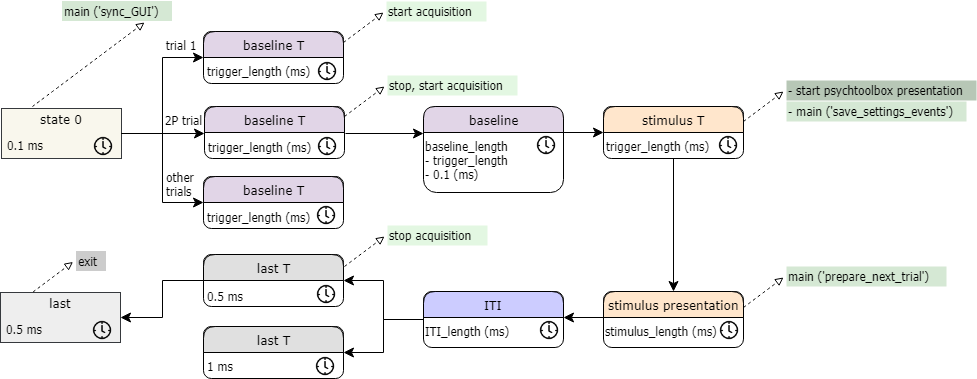
\includegraphics[width=1\linewidth]{3.Chapter/bpodimplementation.png}
	\caption[c1]{Flowchart of the states matrix implemented for the three developed protocols (RF, Tuning and SM). Each state is represented by a name, a timer, state change conditions and output actions. The states machine is formed by three principal states: a baseline, a stimulus display and an ITI. Trigger ("T") states were added, with \textit{trigger length} times corresponding to the duration of the according pulse. All of the state changes were to happen at the end of the internal timer at the current state. The output actions are represented by dashed arrow lines: these represent triggers to the imaging computer (lighter green) through BNC connections, to the NIDAQ of the psychtoolbox matlab instance (darker green) through a wire connection and internal triggers to other functions in the governing machine, through USB connected softcodes (medium green).}
	\label{fig:bpodimplementation}
\end{figure}

After this \textit{submit} process, the user can initiate the psychtoolbox script written for the given protocol at use, in a second matlab instance. This script opens the NIDAQ device and configures it to receive triggers, then opens the screen in the setup monitor in front of the mouse, and loads the session settings in the \textit{next stimulus} file. 

In the case of the RF protocol, this computes a checkerboard mask and divides it into a mask for each grid cell's position figure. It also prepares full screen moving gratings at the settings' frequencies and contrast levels, going in the indicated sequenced directions, within a set of frames in the required number for completing the time length of the stimulus presentation, acording to the monitor's frame rate. Finally, these are combined into textures - sequences of images - that correspond to each trial type and that are saved in a structure for that trial type and every frame of that trial.

The preparation of display movies for the Tuning protocol is done in a similar way: Masks are produced for a circular patch with the possibly multiple sizes and centre positions indicated in the stimulus file, and full screen moving gratings are computed in the brightness levels specified, and for the spatial and temporal frequencies at hand, which can also be more than one in the same session. Then the gratings are masked, forming sets of images (textures), each corresponding to a type of trial and saved in a structure.

For the SM protocol, five masks are produced with the sizes and positions indicated, one circular patch for the center stimuli, and four cardinal quarter-torus for the surround patches. Gratings are drawn at the instructed frequencies and contrasts, also in full-screen. This means that the final textures, maskings of the moving gratings, form in-phase center and surround patches with the same grating properties. These textures regard combinations of the center and surround patches, and each is saved in correspondence to one trial type.

When a trigger reaches the entrance specified in the NIDAQ device, the corresponding trial texture frames are drawn in sequence and the timing between the previous trigger and the current one is displayed on the matlab command window for monitoring possible skipped triggers.

When the textures are loaded, the user can click the start button, which first saves the submitted settings in a stimulus file and then calls the states matrix to run.

Softcodes sent from the bpod device to the governing machine allow processing of given instructions, while the states matrix is simultaneously being run, thus enabling parallel actions. 

As represented in image \ref{fig:bpodimplementation}, in the beginning of a trial, a trigger from the bpod device to the governing machine dictates the GUI's synchronization, updating the displays to the current trial properties. Another softcode is sent, before the stimulus presentation, to save the events and time stamps from the previous trial in a file in the governing machine, in the case of trials after the first. Finally, a \textit{prepare next trial} instruction is sent in the middle of each trial. In parallel to the stimulus presentation, this instruction internally increments the current trial variable, then runs the \textit{set next stimulus} support function and calls the \textit{prepare next matrix} function. This ensures that the next trial variables, GUI and matrix are ready when the current trial finishes and the next \textit{run states matrix} instruction is sent.

During the trials, triggers are sent to the imaging computer to acquire  sequenced images of the animal's brain. The user can decide how many trials are added in every recorded set of images, by changing a GUI variable. Thus, at the beginning of the first trial, a \textit{start acquisition} trigger is sent to the two-photon system and then, at the beginning of every first trial of the imaging sequence, a\textit{next acquisition} trigger is sent, to stop the recording of the images in the previous set and a \textit{start acquisition} follows to record the next images in a new set. A displayed variable in bpod is incremented every time these first trials are reached. In combination with a scanImage interface's display of the number of acquisitions held, the user can monitor the synchronization between bpod and the imaging system.

Once the current trial reaches the last state and the current matrix is finished, the main's \textit{trial completed} function is called. This increments the current trial variable and calls the run states matrix function again. The system enters the prepared states matrix, with the variables, GUI and matrix timings and conditions correspondent to the incremented trial.

The recurrent cycle continues until the last trial is completed, in which case the run states matrix instruction is not sent again, the events and trial stamps from this last trial are saved, and the bpod protocol stops. 

At this point the psychtoolbox script will also finish and the timings displayed in respect to the intervals between triggers can also be saved.

In addition, the bpod protocol can be paused, restarted or stopped at any point. The pause instruction is handled at the beginning of a new trial and, when restarted or stopped, the settings, events and time stamps from the interrupted session are saved, to still retain this information for possible analysis.

In summary, a session runs through sequenced trial matrices. Each of these is created in advance, simultaneously to the running of the preceding matrix. At each trial and state, bpod sends the appropriate triggers to the two photon system for image acquisition, and to the NIDAQ device, for stimulus presentation. In addition, bpod also sends triggers to the governing machine for parallel processing: updating the GUI displays, saving information and preparing the next matrix. Image \ref{fig:examplediagram} shows a simplified diagram of an example mini-session of 4 trials with the two-photon image acquisitions being started at every 2 trials.

\begin{figure}[H]
	\centering
		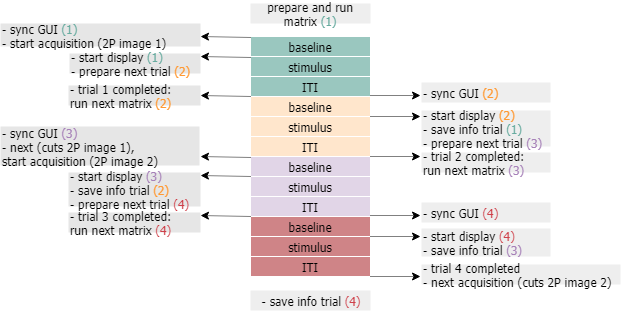
\includegraphics[width=0.8\linewidth]{3.Chapter/examplediagram.png}
	\caption[c1]{Diagram of the simplified states sequence in a session of 4 trials and two-photon acquisition triggers sent every two trials. The gray boxes indicate instructions, and the arrows represent the different trigger instructions sent at the state in its trailing edge. The colored parentesis refer to the trial that each instruction relates to. \label{fig:examplediagram}}
	
\end{figure}